% Created by tikzDevice version 0.11 on 2018-08-15 18:28:12
% !TEX encoding = UTF-8 Unicode
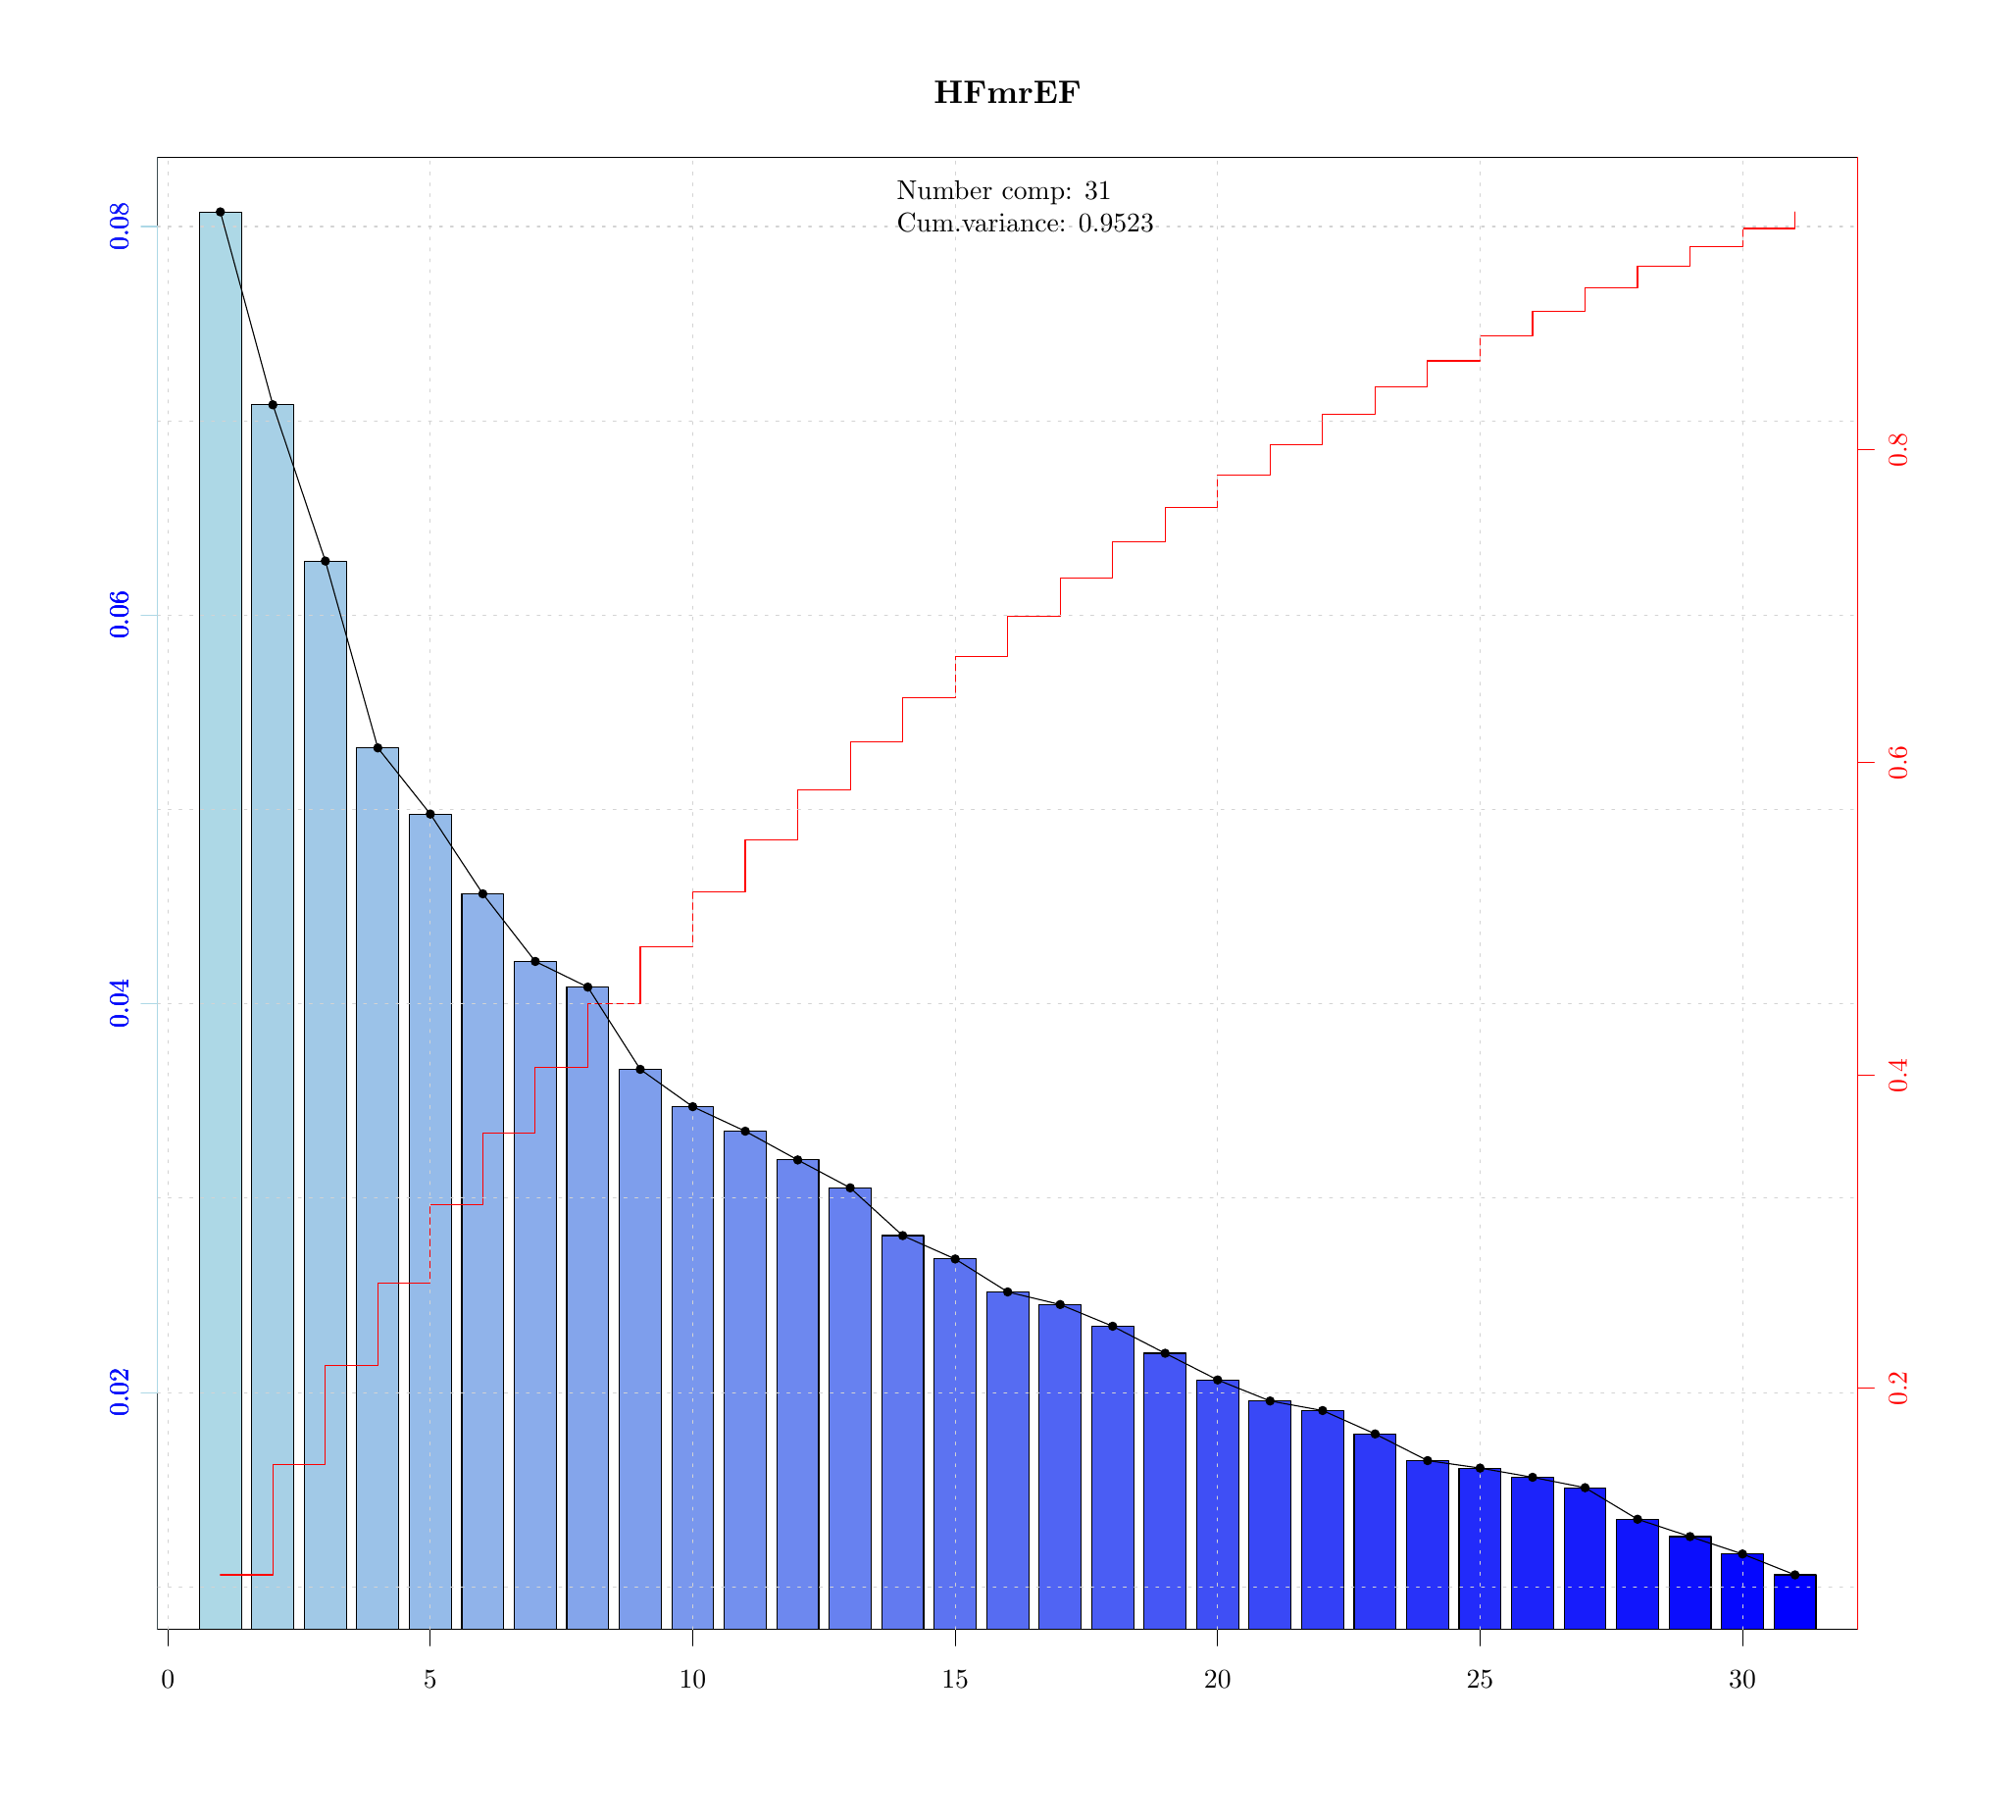
\begin{tikzpicture}[x=1pt,y=1pt]
\definecolor{fillColor}{RGB}{255,255,255}
\path[use as bounding box,fill=fillColor,fill opacity=0.00] (0,0) rectangle (722.70,650.43);
\begin{scope}
\path[clip] ( 48.00, 60.00) rectangle (674.70,602.43);
\definecolor{drawColor}{RGB}{0,0,0}
\definecolor{fillColor}{RGB}{173,216,230}

\path[draw=drawColor,line width= 0.4pt,line join=round,line cap=round,fill=fillColor] ( 63.47, 60.00) rectangle ( 78.95,582.34);
\definecolor{fillColor}{RGB}{167,208,230}

\path[draw=drawColor,line width= 0.4pt,line join=round,line cap=round,fill=fillColor] ( 82.82, 60.00) rectangle ( 98.29,511.25);
\definecolor{fillColor}{RGB}{161,201,231}

\path[draw=drawColor,line width= 0.4pt,line join=round,line cap=round,fill=fillColor] (102.16, 60.00) rectangle (117.63,453.69);
\definecolor{fillColor}{RGB}{155,194,232}

\path[draw=drawColor,line width= 0.4pt,line join=round,line cap=round,fill=fillColor] (121.50, 60.00) rectangle (136.98,384.82);
\definecolor{fillColor}{RGB}{149,187,233}

\path[draw=drawColor,line width= 0.4pt,line join=round,line cap=round,fill=fillColor] (140.84, 60.00) rectangle (156.32,360.44);
\definecolor{fillColor}{RGB}{144,179,234}

\path[draw=drawColor,line width= 0.4pt,line join=round,line cap=round,fill=fillColor] (160.19, 60.00) rectangle (175.66,331.05);
\definecolor{fillColor}{RGB}{138,172,235}

\path[draw=drawColor,line width= 0.4pt,line join=round,line cap=round,fill=fillColor] (179.53, 60.00) rectangle (195.00,306.14);
\definecolor{fillColor}{RGB}{132,165,235}

\path[draw=drawColor,line width= 0.4pt,line join=round,line cap=round,fill=fillColor] (198.87, 60.00) rectangle (214.35,296.68);
\definecolor{fillColor}{RGB}{126,158,236}

\path[draw=drawColor,line width= 0.4pt,line join=round,line cap=round,fill=fillColor] (218.21, 60.00) rectangle (233.69,266.37);
\definecolor{fillColor}{RGB}{121,151,237}

\path[draw=drawColor,line width= 0.4pt,line join=round,line cap=round,fill=fillColor] (237.56, 60.00) rectangle (253.03,252.61);
\definecolor{fillColor}{RGB}{115,144,238}

\path[draw=drawColor,line width= 0.4pt,line join=round,line cap=round,fill=fillColor] (256.90, 60.00) rectangle (272.37,243.59);
\definecolor{fillColor}{RGB}{109,136,239}

\path[draw=drawColor,line width= 0.4pt,line join=round,line cap=round,fill=fillColor] (276.24, 60.00) rectangle (291.72,232.99);
\definecolor{fillColor}{RGB}{103,129,240}

\path[draw=drawColor,line width= 0.4pt,line join=round,line cap=round,fill=fillColor] (295.59, 60.00) rectangle (311.06,222.71);
\definecolor{fillColor}{RGB}{98,122,240}

\path[draw=drawColor,line width= 0.4pt,line join=round,line cap=round,fill=fillColor] (314.93, 60.00) rectangle (330.40,205.11);
\definecolor{fillColor}{RGB}{92,115,241}

\path[draw=drawColor,line width= 0.4pt,line join=round,line cap=round,fill=fillColor] (334.27, 60.00) rectangle (349.74,196.49);
\definecolor{fillColor}{RGB}{86,108,242}

\path[draw=drawColor,line width= 0.4pt,line join=round,line cap=round,fill=fillColor] (353.61, 60.00) rectangle (369.09,184.35);
\definecolor{fillColor}{RGB}{80,100,243}

\path[draw=drawColor,line width= 0.4pt,line join=round,line cap=round,fill=fillColor] (372.96, 60.00) rectangle (388.43,179.71);
\definecolor{fillColor}{RGB}{74,93,244}

\path[draw=drawColor,line width= 0.4pt,line join=round,line cap=round,fill=fillColor] (392.30, 60.00) rectangle (407.77,171.71);
\definecolor{fillColor}{RGB}{69,86,245}

\path[draw=drawColor,line width= 0.4pt,line join=round,line cap=round,fill=fillColor] (411.64, 60.00) rectangle (427.11,161.75);
\definecolor{fillColor}{RGB}{63,79,245}

\path[draw=drawColor,line width= 0.4pt,line join=round,line cap=round,fill=fillColor] (430.98, 60.00) rectangle (446.46,151.93);
\definecolor{fillColor}{RGB}{57,72,246}

\path[draw=drawColor,line width= 0.4pt,line join=round,line cap=round,fill=fillColor] (450.33, 60.00) rectangle (465.80,144.17);
\definecolor{fillColor}{RGB}{51,64,247}

\path[draw=drawColor,line width= 0.4pt,line join=round,line cap=round,fill=fillColor] (469.67, 60.00) rectangle (485.14,140.65);
\definecolor{fillColor}{RGB}{46,57,248}

\path[draw=drawColor,line width= 0.4pt,line join=round,line cap=round,fill=fillColor] (489.01, 60.00) rectangle (504.49,132.03);
\definecolor{fillColor}{RGB}{40,50,249}

\path[draw=drawColor,line width= 0.4pt,line join=round,line cap=round,fill=fillColor] (508.35, 60.00) rectangle (523.83,122.20);
\definecolor{fillColor}{RGB}{34,43,250}

\path[draw=drawColor,line width= 0.4pt,line join=round,line cap=round,fill=fillColor] (527.70, 60.00) rectangle (543.17,119.45);
\definecolor{fillColor}{RGB}{28,35,250}

\path[draw=drawColor,line width= 0.4pt,line join=round,line cap=round,fill=fillColor] (547.04, 60.00) rectangle (562.51,116.05);
\definecolor{fillColor}{RGB}{23,28,251}

\path[draw=drawColor,line width= 0.4pt,line join=round,line cap=round,fill=fillColor] (566.38, 60.00) rectangle (581.86,112.21);
\definecolor{fillColor}{RGB}{17,21,252}

\path[draw=drawColor,line width= 0.4pt,line join=round,line cap=round,fill=fillColor] (585.72, 60.00) rectangle (601.20,100.59);
\definecolor{fillColor}{RGB}{11,14,253}

\path[draw=drawColor,line width= 0.4pt,line join=round,line cap=round,fill=fillColor] (605.07, 60.00) rectangle (620.54, 94.20);
\definecolor{fillColor}{RGB}{5,7,254}

\path[draw=drawColor,line width= 0.4pt,line join=round,line cap=round,fill=fillColor] (624.41, 60.00) rectangle (639.88, 87.79);
\definecolor{fillColor}{RGB}{0,0,255}

\path[draw=drawColor,line width= 0.4pt,line join=round,line cap=round,fill=fillColor] (643.75, 60.00) rectangle (659.23, 80.09);
\end{scope}
\begin{scope}
\path[clip] (  0.00,  0.00) rectangle (722.70,650.43);
\definecolor{drawColor}{RGB}{0,0,0}

\node[text=drawColor,anchor=base,inner sep=0pt, outer sep=0pt, scale=  1.20] at (361.35,622.29) {\bfseries HFmrEF};
\end{scope}
\begin{scope}
\path[clip] (  0.00,  0.00) rectangle (722.70,650.43);
\definecolor{drawColor}{RGB}{0,0,0}

\path[draw=drawColor,line width= 0.4pt,line join=round,line cap=round] ( 48.00, 60.00) --
	(674.70, 60.00) --
	(674.70,602.43) --
	( 48.00,602.43) --
	( 48.00, 60.00);

\path[draw=drawColor,line width= 0.4pt,line join=round,line cap=round] ( 51.87, 60.00) -- (632.15, 60.00);

\path[draw=drawColor,line width= 0.4pt,line join=round,line cap=round] ( 51.87, 60.00) -- ( 51.87, 54.00);

\path[draw=drawColor,line width= 0.4pt,line join=round,line cap=round] (148.58, 60.00) -- (148.58, 54.00);

\path[draw=drawColor,line width= 0.4pt,line join=round,line cap=round] (245.29, 60.00) -- (245.29, 54.00);

\path[draw=drawColor,line width= 0.4pt,line join=round,line cap=round] (342.01, 60.00) -- (342.01, 54.00);

\path[draw=drawColor,line width= 0.4pt,line join=round,line cap=round] (438.72, 60.00) -- (438.72, 54.00);

\path[draw=drawColor,line width= 0.4pt,line join=round,line cap=round] (535.43, 60.00) -- (535.43, 54.00);

\path[draw=drawColor,line width= 0.4pt,line join=round,line cap=round] (632.15, 60.00) -- (632.15, 54.00);

\node[text=drawColor,anchor=base,inner sep=0pt, outer sep=0pt, scale=  1.00] at ( 51.87, 38.40) {0};

\node[text=drawColor,anchor=base,inner sep=0pt, outer sep=0pt, scale=  1.00] at (148.58, 38.40) {5};

\node[text=drawColor,anchor=base,inner sep=0pt, outer sep=0pt, scale=  1.00] at (245.29, 38.40) {10};

\node[text=drawColor,anchor=base,inner sep=0pt, outer sep=0pt, scale=  1.00] at (342.01, 38.40) {15};

\node[text=drawColor,anchor=base,inner sep=0pt, outer sep=0pt, scale=  1.00] at (438.72, 38.40) {20};

\node[text=drawColor,anchor=base,inner sep=0pt, outer sep=0pt, scale=  1.00] at (535.43, 38.40) {25};

\node[text=drawColor,anchor=base,inner sep=0pt, outer sep=0pt, scale=  1.00] at (632.15, 38.40) {30};
\definecolor{drawColor}{RGB}{173,216,230}

\path[draw=drawColor,line width= 0.4pt,line join=round,line cap=round] ( 48.00,147.28) -- ( 48.00,576.95);

\path[draw=drawColor,line width= 0.4pt,line join=round,line cap=round] ( 48.00,147.28) -- ( 42.00,147.28);

\path[draw=drawColor,line width= 0.4pt,line join=round,line cap=round] ( 48.00,290.50) -- ( 42.00,290.50);

\path[draw=drawColor,line width= 0.4pt,line join=round,line cap=round] ( 48.00,433.73) -- ( 42.00,433.73);

\path[draw=drawColor,line width= 0.4pt,line join=round,line cap=round] ( 48.00,576.95) -- ( 42.00,576.95);

\node[text=drawColor,rotate= 90.00,anchor=base,inner sep=0pt, outer sep=0pt, scale=  1.00] at ( 37.20,147.28) {0.02};
\definecolor{drawColor}{RGB}{167,208,230}

\node[text=drawColor,rotate= 90.00,anchor=base,inner sep=0pt, outer sep=0pt, scale=  1.00] at ( 37.20,290.50) {0.04};
\definecolor{drawColor}{RGB}{161,201,231}

\node[text=drawColor,rotate= 90.00,anchor=base,inner sep=0pt, outer sep=0pt, scale=  1.00] at ( 37.20,433.73) {0.06};
\definecolor{drawColor}{RGB}{155,194,232}

\node[text=drawColor,rotate= 90.00,anchor=base,inner sep=0pt, outer sep=0pt, scale=  1.00] at ( 37.20,576.95) {0.08};
\definecolor{drawColor}{RGB}{149,187,233}

\node[text=drawColor,rotate= 90.00,anchor=base,inner sep=0pt, outer sep=0pt, scale=  1.00] at ( 37.20,147.28) {0.02};
\definecolor{drawColor}{RGB}{144,179,234}

\node[text=drawColor,rotate= 90.00,anchor=base,inner sep=0pt, outer sep=0pt, scale=  1.00] at ( 37.20,290.50) {0.04};
\definecolor{drawColor}{RGB}{138,172,235}

\node[text=drawColor,rotate= 90.00,anchor=base,inner sep=0pt, outer sep=0pt, scale=  1.00] at ( 37.20,433.73) {0.06};
\definecolor{drawColor}{RGB}{132,165,235}

\node[text=drawColor,rotate= 90.00,anchor=base,inner sep=0pt, outer sep=0pt, scale=  1.00] at ( 37.20,576.95) {0.08};
\definecolor{drawColor}{RGB}{126,158,236}

\node[text=drawColor,rotate= 90.00,anchor=base,inner sep=0pt, outer sep=0pt, scale=  1.00] at ( 37.20,147.28) {0.02};
\definecolor{drawColor}{RGB}{121,151,237}

\node[text=drawColor,rotate= 90.00,anchor=base,inner sep=0pt, outer sep=0pt, scale=  1.00] at ( 37.20,290.50) {0.04};
\definecolor{drawColor}{RGB}{115,144,238}

\node[text=drawColor,rotate= 90.00,anchor=base,inner sep=0pt, outer sep=0pt, scale=  1.00] at ( 37.20,433.73) {0.06};
\definecolor{drawColor}{RGB}{109,136,239}

\node[text=drawColor,rotate= 90.00,anchor=base,inner sep=0pt, outer sep=0pt, scale=  1.00] at ( 37.20,576.95) {0.08};
\definecolor{drawColor}{RGB}{103,129,240}

\node[text=drawColor,rotate= 90.00,anchor=base,inner sep=0pt, outer sep=0pt, scale=  1.00] at ( 37.20,147.28) {0.02};
\definecolor{drawColor}{RGB}{98,122,240}

\node[text=drawColor,rotate= 90.00,anchor=base,inner sep=0pt, outer sep=0pt, scale=  1.00] at ( 37.20,290.50) {0.04};
\definecolor{drawColor}{RGB}{92,115,241}

\node[text=drawColor,rotate= 90.00,anchor=base,inner sep=0pt, outer sep=0pt, scale=  1.00] at ( 37.20,433.73) {0.06};
\definecolor{drawColor}{RGB}{86,108,242}

\node[text=drawColor,rotate= 90.00,anchor=base,inner sep=0pt, outer sep=0pt, scale=  1.00] at ( 37.20,576.95) {0.08};
\definecolor{drawColor}{RGB}{80,100,243}

\node[text=drawColor,rotate= 90.00,anchor=base,inner sep=0pt, outer sep=0pt, scale=  1.00] at ( 37.20,147.28) {0.02};
\definecolor{drawColor}{RGB}{74,93,244}

\node[text=drawColor,rotate= 90.00,anchor=base,inner sep=0pt, outer sep=0pt, scale=  1.00] at ( 37.20,290.50) {0.04};
\definecolor{drawColor}{RGB}{69,86,245}

\node[text=drawColor,rotate= 90.00,anchor=base,inner sep=0pt, outer sep=0pt, scale=  1.00] at ( 37.20,433.73) {0.06};
\definecolor{drawColor}{RGB}{63,79,245}

\node[text=drawColor,rotate= 90.00,anchor=base,inner sep=0pt, outer sep=0pt, scale=  1.00] at ( 37.20,576.95) {0.08};
\definecolor{drawColor}{RGB}{57,72,246}

\node[text=drawColor,rotate= 90.00,anchor=base,inner sep=0pt, outer sep=0pt, scale=  1.00] at ( 37.20,147.28) {0.02};
\definecolor{drawColor}{RGB}{51,64,247}

\node[text=drawColor,rotate= 90.00,anchor=base,inner sep=0pt, outer sep=0pt, scale=  1.00] at ( 37.20,290.50) {0.04};
\definecolor{drawColor}{RGB}{46,57,248}

\node[text=drawColor,rotate= 90.00,anchor=base,inner sep=0pt, outer sep=0pt, scale=  1.00] at ( 37.20,433.73) {0.06};
\definecolor{drawColor}{RGB}{40,50,249}

\node[text=drawColor,rotate= 90.00,anchor=base,inner sep=0pt, outer sep=0pt, scale=  1.00] at ( 37.20,576.95) {0.08};
\definecolor{drawColor}{RGB}{34,43,250}

\node[text=drawColor,rotate= 90.00,anchor=base,inner sep=0pt, outer sep=0pt, scale=  1.00] at ( 37.20,147.28) {0.02};
\definecolor{drawColor}{RGB}{28,35,250}

\node[text=drawColor,rotate= 90.00,anchor=base,inner sep=0pt, outer sep=0pt, scale=  1.00] at ( 37.20,290.50) {0.04};
\definecolor{drawColor}{RGB}{23,28,251}

\node[text=drawColor,rotate= 90.00,anchor=base,inner sep=0pt, outer sep=0pt, scale=  1.00] at ( 37.20,433.73) {0.06};
\definecolor{drawColor}{RGB}{17,21,252}

\node[text=drawColor,rotate= 90.00,anchor=base,inner sep=0pt, outer sep=0pt, scale=  1.00] at ( 37.20,576.95) {0.08};
\definecolor{drawColor}{RGB}{11,14,253}

\node[text=drawColor,rotate= 90.00,anchor=base,inner sep=0pt, outer sep=0pt, scale=  1.00] at ( 37.20,147.28) {0.02};
\definecolor{drawColor}{RGB}{5,7,254}

\node[text=drawColor,rotate= 90.00,anchor=base,inner sep=0pt, outer sep=0pt, scale=  1.00] at ( 37.20,290.50) {0.04};
\definecolor{drawColor}{RGB}{0,0,255}

\node[text=drawColor,rotate= 90.00,anchor=base,inner sep=0pt, outer sep=0pt, scale=  1.00] at ( 37.20,433.73) {0.06};
\end{scope}
\begin{scope}
\path[clip] ( 48.00, 60.00) rectangle (674.70,602.43);
\definecolor{drawColor}{RGB}{173,216,230}

\path[draw=drawColor,line width= 0.4pt,line join=round,line cap=round] ( 48.00, 60.00) -- ( 48.00,602.43);
\definecolor{drawColor}{RGB}{255,0,0}

\path[draw=drawColor,line width= 0.4pt,line join=round,line cap=round] ( 71.21, 80.09) --
	( 90.55, 80.09) --
	( 90.55,120.91) --
	(109.90,120.91) --
	(109.90,157.09) --
	(129.24,157.09) --
	(129.24,187.73) --
	(148.58,187.73) --
	(148.58,216.41) --
	(167.92,216.41) --
	(167.92,242.73) --
	(187.27,242.73) --
	(187.27,267.04) --
	(206.61,267.04) --
	(206.61,290.59) --
	(225.95,290.59) --
	(225.95,311.70) --
	(245.29,311.70) --
	(245.29,331.70) --
	(264.64,331.70) --
	(264.64,350.97) --
	(283.98,350.97) --
	(283.98,369.40) --
	(303.32,369.40) --
	(303.32,386.99) --
	(322.66,386.99) --
	(322.66,403.17) --
	(342.01,403.17) --
	(342.01,418.66) --
	(361.35,418.66) --
	(361.35,433.17) --
	(380.69,433.17) --
	(380.69,447.30) --
	(400.04,447.30) --
	(400.04,460.79) --
	(419.38,460.79) --
	(419.38,473.49) --
	(438.72,473.49) --
	(438.72,485.39) --
	(458.06,485.39) --
	(458.06,496.66) --
	(477.41,496.66) --
	(477.41,507.65) --
	(496.75,507.65) --
	(496.75,517.95) --
	(516.09,517.95) --
	(516.09,527.46) --
	(535.43,527.46) --
	(535.43,536.75) --
	(554.78,536.75) --
	(554.78,545.76) --
	(574.12,545.76) --
	(574.12,554.46) --
	(593.46,554.46) --
	(593.46,562.23) --
	(612.80,562.23) --
	(612.80,569.48) --
	(632.15,569.48) --
	(632.15,576.22) --
	(651.49,576.22) --
	(651.49,582.34);
\end{scope}
\begin{scope}
\path[clip] (  0.00,  0.00) rectangle (722.70,650.43);
\definecolor{drawColor}{RGB}{255,0,0}

\path[draw=drawColor,line width= 0.4pt,line join=round,line cap=round] (674.70,148.81) -- (674.70,494.59);

\path[draw=drawColor,line width= 0.4pt,line join=round,line cap=round] (674.70,148.81) -- (680.70,148.81);

\path[draw=drawColor,line width= 0.4pt,line join=round,line cap=round] (674.70,264.07) -- (680.70,264.07);

\path[draw=drawColor,line width= 0.4pt,line join=round,line cap=round] (674.70,379.33) -- (680.70,379.33);

\path[draw=drawColor,line width= 0.4pt,line join=round,line cap=round] (674.70,494.59) -- (680.70,494.59);

\node[text=drawColor,rotate= 90.00,anchor=base,inner sep=0pt, outer sep=0pt, scale=  1.00] at (692.70,148.81) {0.2};

\node[text=drawColor,rotate= 90.00,anchor=base,inner sep=0pt, outer sep=0pt, scale=  1.00] at (692.70,264.07) {0.4};

\node[text=drawColor,rotate= 90.00,anchor=base,inner sep=0pt, outer sep=0pt, scale=  1.00] at (692.70,379.33) {0.6};

\node[text=drawColor,rotate= 90.00,anchor=base,inner sep=0pt, outer sep=0pt, scale=  1.00] at (692.70,494.59) {0.8};
\end{scope}
\begin{scope}
\path[clip] ( 48.00, 60.00) rectangle (674.70,602.43);
\definecolor{drawColor}{RGB}{255,0,0}

\path[draw=drawColor,line width= 0.4pt,line join=round,line cap=round] (674.70, 60.00) -- (674.70,602.43);
\definecolor{drawColor}{RGB}{211,211,211}

\path[draw=drawColor,line width= 0.4pt,dash pattern=on 1pt off 3pt ,line join=round,line cap=round] ( 51.87, 60.00) -- ( 51.87,602.43);

\path[draw=drawColor,line width= 0.4pt,dash pattern=on 1pt off 3pt ,line join=round,line cap=round] (148.58, 60.00) -- (148.58,602.43);

\path[draw=drawColor,line width= 0.4pt,dash pattern=on 1pt off 3pt ,line join=round,line cap=round] (245.29, 60.00) -- (245.29,602.43);

\path[draw=drawColor,line width= 0.4pt,dash pattern=on 1pt off 3pt ,line join=round,line cap=round] (342.01, 60.00) -- (342.01,602.43);

\path[draw=drawColor,line width= 0.4pt,dash pattern=on 1pt off 3pt ,line join=round,line cap=round] (438.72, 60.00) -- (438.72,602.43);

\path[draw=drawColor,line width= 0.4pt,dash pattern=on 1pt off 3pt ,line join=round,line cap=round] (535.43, 60.00) -- (535.43,602.43);

\path[draw=drawColor,line width= 0.4pt,dash pattern=on 1pt off 3pt ,line join=round,line cap=round] (632.15, 60.00) -- (632.15,602.43);

\path[draw=drawColor,line width= 0.4pt,dash pattern=on 1pt off 3pt ,line join=round,line cap=round] ( 48.00, 75.67) -- (674.70, 75.67);

\path[draw=drawColor,line width= 0.4pt,dash pattern=on 1pt off 3pt ,line join=round,line cap=round] ( 48.00,147.28) -- (674.70,147.28);

\path[draw=drawColor,line width= 0.4pt,dash pattern=on 1pt off 3pt ,line join=round,line cap=round] ( 48.00,218.89) -- (674.70,218.89);

\path[draw=drawColor,line width= 0.4pt,dash pattern=on 1pt off 3pt ,line join=round,line cap=round] ( 48.00,290.50) -- (674.70,290.50);

\path[draw=drawColor,line width= 0.4pt,dash pattern=on 1pt off 3pt ,line join=round,line cap=round] ( 48.00,362.11) -- (674.70,362.11);

\path[draw=drawColor,line width= 0.4pt,dash pattern=on 1pt off 3pt ,line join=round,line cap=round] ( 48.00,433.73) -- (674.70,433.73);

\path[draw=drawColor,line width= 0.4pt,dash pattern=on 1pt off 3pt ,line join=round,line cap=round] ( 48.00,505.34) -- (674.70,505.34);

\path[draw=drawColor,line width= 0.4pt,dash pattern=on 1pt off 3pt ,line join=round,line cap=round] ( 48.00,576.95) -- (674.70,576.95);
\definecolor{drawColor}{RGB}{0,0,0}

\path[draw=drawColor,line width= 0.4pt,line join=round,line cap=round] ( 71.21,582.34) --
	( 90.55,511.25) --
	(109.90,453.69) --
	(129.24,384.82) --
	(148.58,360.44) --
	(167.92,331.05) --
	(187.27,306.14) --
	(206.61,296.68) --
	(225.95,266.37) --
	(245.29,252.61) --
	(264.64,243.59) --
	(283.98,232.99) --
	(303.32,222.71) --
	(322.66,205.11) --
	(342.01,196.49) --
	(361.35,184.35) --
	(380.69,179.71) --
	(400.04,171.71) --
	(419.38,161.75) --
	(438.72,151.93) --
	(458.06,144.17) --
	(477.41,140.65) --
	(496.75,132.03) --
	(516.09,122.20) --
	(535.43,119.45) --
	(554.78,116.05) --
	(574.12,112.21) --
	(593.46,100.59) --
	(612.80, 94.20) --
	(632.15, 87.79) --
	(651.49, 80.09);
\definecolor{fillColor}{RGB}{0,0,0}

\path[draw=drawColor,line width= 0.4pt,line join=round,line cap=round,fill=fillColor] ( 71.21,582.34) circle (  1.50);

\path[draw=drawColor,line width= 0.4pt,line join=round,line cap=round,fill=fillColor] ( 90.55,511.25) circle (  1.50);

\path[draw=drawColor,line width= 0.4pt,line join=round,line cap=round,fill=fillColor] (109.90,453.69) circle (  1.50);

\path[draw=drawColor,line width= 0.4pt,line join=round,line cap=round,fill=fillColor] (129.24,384.82) circle (  1.50);

\path[draw=drawColor,line width= 0.4pt,line join=round,line cap=round,fill=fillColor] (148.58,360.44) circle (  1.50);

\path[draw=drawColor,line width= 0.4pt,line join=round,line cap=round,fill=fillColor] (167.92,331.05) circle (  1.50);

\path[draw=drawColor,line width= 0.4pt,line join=round,line cap=round,fill=fillColor] (187.27,306.14) circle (  1.50);

\path[draw=drawColor,line width= 0.4pt,line join=round,line cap=round,fill=fillColor] (206.61,296.68) circle (  1.50);

\path[draw=drawColor,line width= 0.4pt,line join=round,line cap=round,fill=fillColor] (225.95,266.37) circle (  1.50);

\path[draw=drawColor,line width= 0.4pt,line join=round,line cap=round,fill=fillColor] (245.29,252.61) circle (  1.50);

\path[draw=drawColor,line width= 0.4pt,line join=round,line cap=round,fill=fillColor] (264.64,243.59) circle (  1.50);

\path[draw=drawColor,line width= 0.4pt,line join=round,line cap=round,fill=fillColor] (283.98,232.99) circle (  1.50);

\path[draw=drawColor,line width= 0.4pt,line join=round,line cap=round,fill=fillColor] (303.32,222.71) circle (  1.50);

\path[draw=drawColor,line width= 0.4pt,line join=round,line cap=round,fill=fillColor] (322.66,205.11) circle (  1.50);

\path[draw=drawColor,line width= 0.4pt,line join=round,line cap=round,fill=fillColor] (342.01,196.49) circle (  1.50);

\path[draw=drawColor,line width= 0.4pt,line join=round,line cap=round,fill=fillColor] (361.35,184.35) circle (  1.50);

\path[draw=drawColor,line width= 0.4pt,line join=round,line cap=round,fill=fillColor] (380.69,179.71) circle (  1.50);

\path[draw=drawColor,line width= 0.4pt,line join=round,line cap=round,fill=fillColor] (400.04,171.71) circle (  1.50);

\path[draw=drawColor,line width= 0.4pt,line join=round,line cap=round,fill=fillColor] (419.38,161.75) circle (  1.50);

\path[draw=drawColor,line width= 0.4pt,line join=round,line cap=round,fill=fillColor] (438.72,151.93) circle (  1.50);

\path[draw=drawColor,line width= 0.4pt,line join=round,line cap=round,fill=fillColor] (458.06,144.17) circle (  1.50);

\path[draw=drawColor,line width= 0.4pt,line join=round,line cap=round,fill=fillColor] (477.41,140.65) circle (  1.50);

\path[draw=drawColor,line width= 0.4pt,line join=round,line cap=round,fill=fillColor] (496.75,132.03) circle (  1.50);

\path[draw=drawColor,line width= 0.4pt,line join=round,line cap=round,fill=fillColor] (516.09,122.20) circle (  1.50);

\path[draw=drawColor,line width= 0.4pt,line join=round,line cap=round,fill=fillColor] (535.43,119.45) circle (  1.50);

\path[draw=drawColor,line width= 0.4pt,line join=round,line cap=round,fill=fillColor] (554.78,116.05) circle (  1.50);

\path[draw=drawColor,line width= 0.4pt,line join=round,line cap=round,fill=fillColor] (574.12,112.21) circle (  1.50);

\path[draw=drawColor,line width= 0.4pt,line join=round,line cap=round,fill=fillColor] (593.46,100.59) circle (  1.50);

\path[draw=drawColor,line width= 0.4pt,line join=round,line cap=round,fill=fillColor] (612.80, 94.20) circle (  1.50);

\path[draw=drawColor,line width= 0.4pt,line join=round,line cap=round,fill=fillColor] (632.15, 87.79) circle (  1.50);

\path[draw=drawColor,line width= 0.4pt,line join=round,line cap=round,fill=fillColor] (651.49, 80.09) circle (  1.50);

\node[text=drawColor,anchor=base west,inner sep=0pt, outer sep=0pt, scale=  1.00] at (320.51,586.93) {Number comp: 31};

\node[text=drawColor,anchor=base west,inner sep=0pt, outer sep=0pt, scale=  1.00] at (320.51,574.88) {Cum.variance: 0.9523};
\end{scope}
\end{tikzpicture}
